\documentclass[11pt]{exam}
\usepackage{tikz}
\usetikzlibrary {plotmarks}
\usepackage{multicol}
\usepackage{subfigure}

\newcommand{\class}{MATH 96}
\newcommand{\term}{Fall 2024}
\newcommand{\examnum}{Exam 2} 
\newcommand{\examdate}{10/30/24}
\newcommand{\timelimit}{60 Minutes}

\parindent 0ex

\begin{document} 

\pagestyle{head}
\firstpageheader{}{}{}
\runningheader{\class}{\examnum\ - Page \thepage\ of \numpages}{\examdate}
\runningheadrule

\begin{flushright}
\begin{tabular}{p{2.2in} r l}
\textbf{\class} & \textbf{Name:}     & \makebox[2.7in]{\hrulefill}\\
\textbf{\term}  &                    &\\
\textbf{\examnum} &  & \\
 & \textbf{Section:} & \makebox[2.7in]{\hrulefill}\\

\end{tabular}\\
\end{flushright}
\rule[1ex]{\textwidth}{.1pt}

This exam contains \numpages\ pages (including this cover page) and
\numquestions\ problems.  Check to see if any pages are missing.  Enter
your name and your section above.
\vspace{0.2in}

You may \emph{not} use textbooks, course notes, cell phones, or calculators during this exam.
\vspace{0.2in}

You are required to show your work on each problem on this exam, and the following rules apply:
\vspace{0.2in}

\begin{minipage}[t]{3.7in}
\vspace{0pt}
\begin{itemize}

\item \textbf{Organize your work in a reasonable, neat, and coherent way.} Work that is jumbled, disorganized, or lacks clear reasoning will receive little credit.  

\item \textbf{Partial credit may be given.} Any answer must be supported by calculations, explanation, and/or algebraic work to receive full credit.  Unsupported answers will not receive full credit, but well-argued, incorrect solutions may earn partial credit.

\item \textbf{If you require more space, use the back of a page.} Clearly indicate when you do this below the problem.
\end{itemize}

Do not write in the table to the right.
\end{minipage}
\hfill
\begin{minipage}[t]{2.3in}
\vspace{0pt}
\gradetablestretch{2}
\vqword{Problem}
\addpoints
\gradetable[v][pages]
\end{minipage}
%=======================================================================================================================
\newpage
\begin{questions}

%=======================================================================================================================
\question[20] Find solutions to the given linear inequalities and express the solution sets using both interval notation and number line representation.

\noaddpoints
\begin{parts}
\part[10] $\displaystyle -3 x - 2 > -x - 4$
\vspace{2.2in}

Solution set in interval notation:

\vspace{.3in}
Solution set on the number line:

\vspace{.3in}
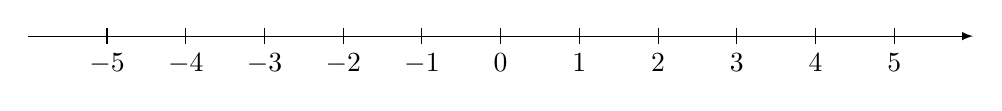
\begin{tikzpicture}
  % Draw the axis line
  \draw[-latex] (-6,0) -- (6,0);
  
  % Draw tick marks and labels
  \foreach \x in {-5,...,5}
    \draw (\x,0.1) -- (\x,-0.1) node[below] {$\x$};
\end{tikzpicture}
\vspace{.5in}

\part[10] $\displaystyle x + 10 \geq -\frac{3}{2}x$
\vspace{2.2in}

Solution set in interval notation:

\vspace{.3in}
Solution set on the number line:

\vspace{.3in}
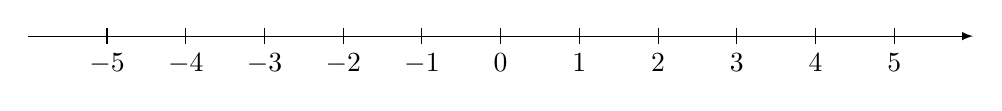
\begin{tikzpicture}
  % Draw the axis line
  \draw[-latex] (-6,0) -- (6,0);
  
  % Draw tick marks and labels
  \foreach \x in {-5,...,5}
    \draw (\x,0.1) -- (\x,-0.1) node[below] {$\x$};
\end{tikzpicture}
\vspace{0.1in}

\end{parts}
\addpoints

\question[16] Decide whether each equation is \emph{true}(T) or \emph{false}(F). Provide a brief explanation if it is found to be \emph{false.}
\noaddpoints
\begin{parts}
\begin{multicols}{2}
\part $\displaystyle (-2)^{3} = -8$

\part $\displaystyle \frac{3^{-1}}{3^{-3}} = 9$
\end{multicols}
\vspace{1in}

\begin{multicols}{2}
\part $\displaystyle (4^{-2})^{-1} = 4^{2}$

\part $\displaystyle \frac{64}{27} = \left(\frac{4}{3}\right)^{3}$
\end{multicols}
\vspace{1in}

\begin{multicols}{2}
\part $\displaystyle 2^{-3} = -\frac{1}{8}$

\part $\displaystyle (6^3)^{-2} = \frac{1}{6^6}$
\end{multicols}
\vspace{1in}
\addpoints
\end{parts}

\question[12] Solve~~$\displaystyle \frac{1}{3}\left\vert 2x - 5 \right\vert = 4$.
\newpage
%==============================================================================================================
\question[16] Simplify each expression as much as possible, ensuring all exponents are \textbf{positive}.
\noaddpoints
\vspace{2pt}

\begin{parts}
\begin{multicols}{2}
\part[8] $\displaystyle \frac{6m^{-2}n^4}{3m^3n}$
\part[8] $\displaystyle \left(\frac{5x^{-1}y^2}{10x^3y^{-1}}\right)^{-1}$ 
\end{multicols}
\end{parts}
\vspace{2.5in}
\addpoints
\question[16] Find solutions to the given inequalities and express the solution sets using interval notation.
\noaddpoints
\begin{parts}

\part[8] $\displaystyle 5 < 3|x + 2| $

\vspace{2.5in}
\part[8] $\displaystyle -7 \le 4x + 1 < 9$

\vspace{2.5in}

\end{parts}
\addpoints
\newpage

\question[20] The Madison Forward soccer team sells 600 tickets for a competition at Breese Stevens Field. Children's tickets cost \$5, and adult tickets cost \$15. The Madison Forward team made \$7000 in ticket sales that day. How many children's and adult tickets did they sell?

\noaddpoints
\begin{parts}
\part[4] Let $x$ be the number of children's tickets and $y$ be the number of adult tickets. Set up the system of two linear equations involving $x$ and $y$.

\vspace{2in}

\part[8] Solve the system of two linear equations using the addition/elimination method.
\vspace{3in}

\part[8] Solve the system of two linear equations using the substitution method.
\vspace{3in}

\end{parts}
\addpoints

\end{questions}
\end{document}


